
\section{Cell grid}
\label{sec:grid}

\begin{frame}
    \frametitle{Linking cells in a grid}
    3D vector matrix of \texttt{std::unique\_ptr} to cells
    \begin{itemize}
        \item Initialization through specifications in XML file
        \item Assigns particle references of cells to particles in the particle container
        \item \textbf{Key function:} Get indices of relevant neighbor cells
    \end{itemize}
\end{frame}

\begin{frame}
    \frametitle{getNeighborCells}
    Algorithm to utilize newton's third law needed on cell iteration level!\newline
    $\longrightarrow$ \texttt{std::list<CellIndex> getNeighborCells(const Cellindex)}
    \begin{itemize}
        \item Distinguish between neighbor pairs, that already have been included in calculations
        \item Given an index to a cell, iteration over each neighboring cell
        \item If \textbf{neighbor cell's counter = 0}: Increment parameter cell's counter and add neighbor cell's index to return list
        \item If \textbf{neighbor cell's counter $>$ 0}: Decrease neighbor cell's counter and ignore the cell.
    \end{itemize}
\end{frame}

\begin{frame}
    \frametitle{Algorithm of getting neighbor indices}
    \begin{figure}
        \label{fig:neighbor}
        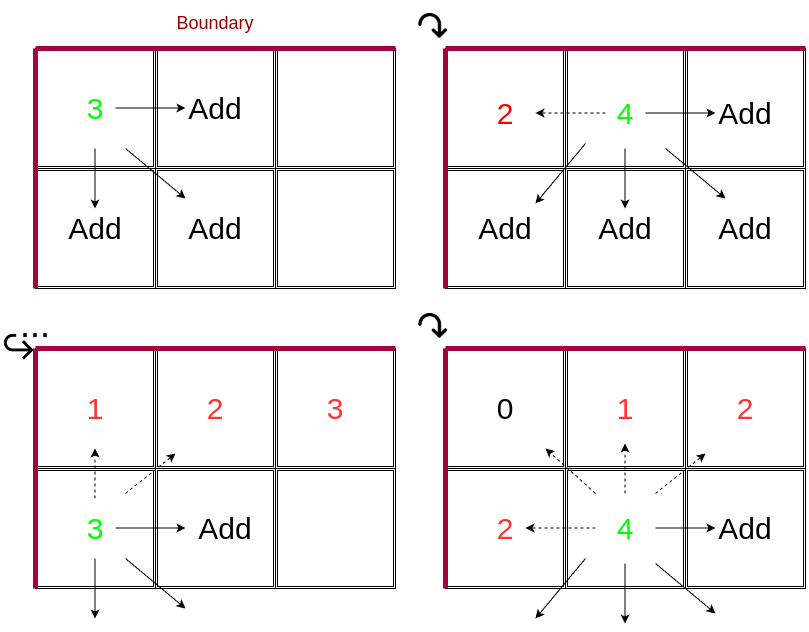
\includegraphics[width=0.6\textwidth]{res/getNeighbor.drawio}
    \end{figure}
\end{frame}

\begin{frame}
    \frametitle{Project Expansion}
    \begin{figure}
        \label{fig:umlcellgrid}
        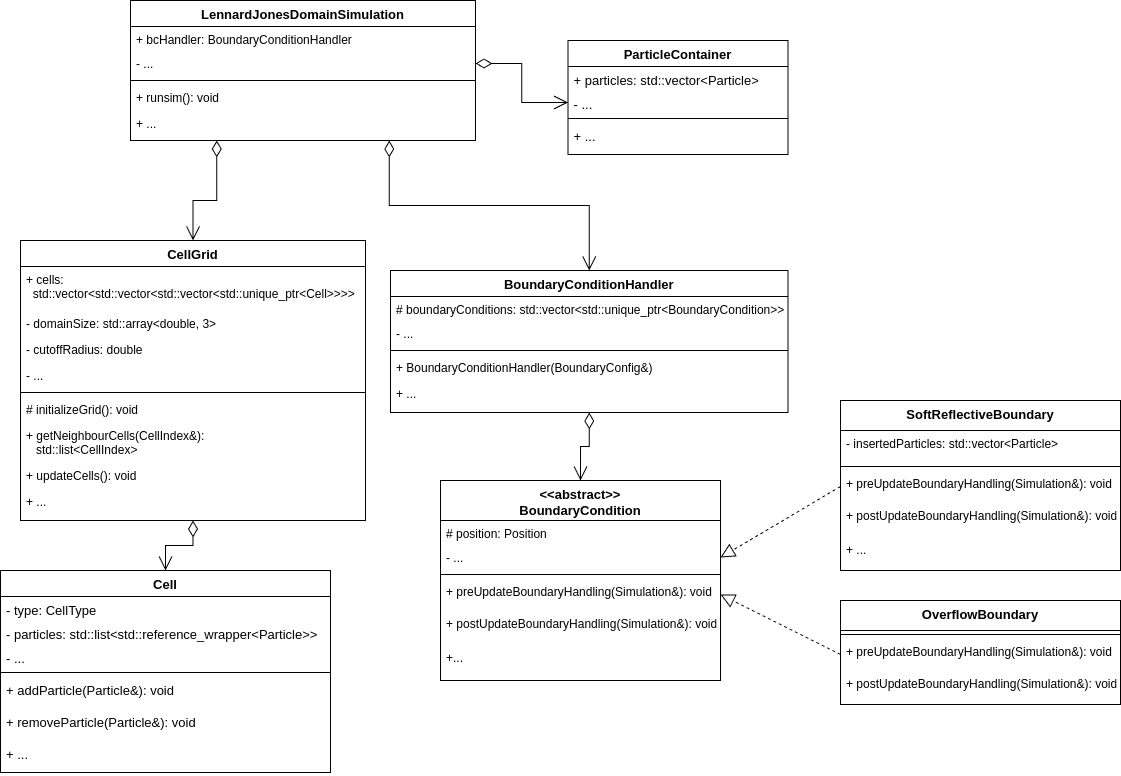
\includegraphics[width=0.7\textwidth]{res/UML3.drawio}
    \end{figure}
\end{frame}